\subsection{Data}

\begin{figure}[H]
    \centering
    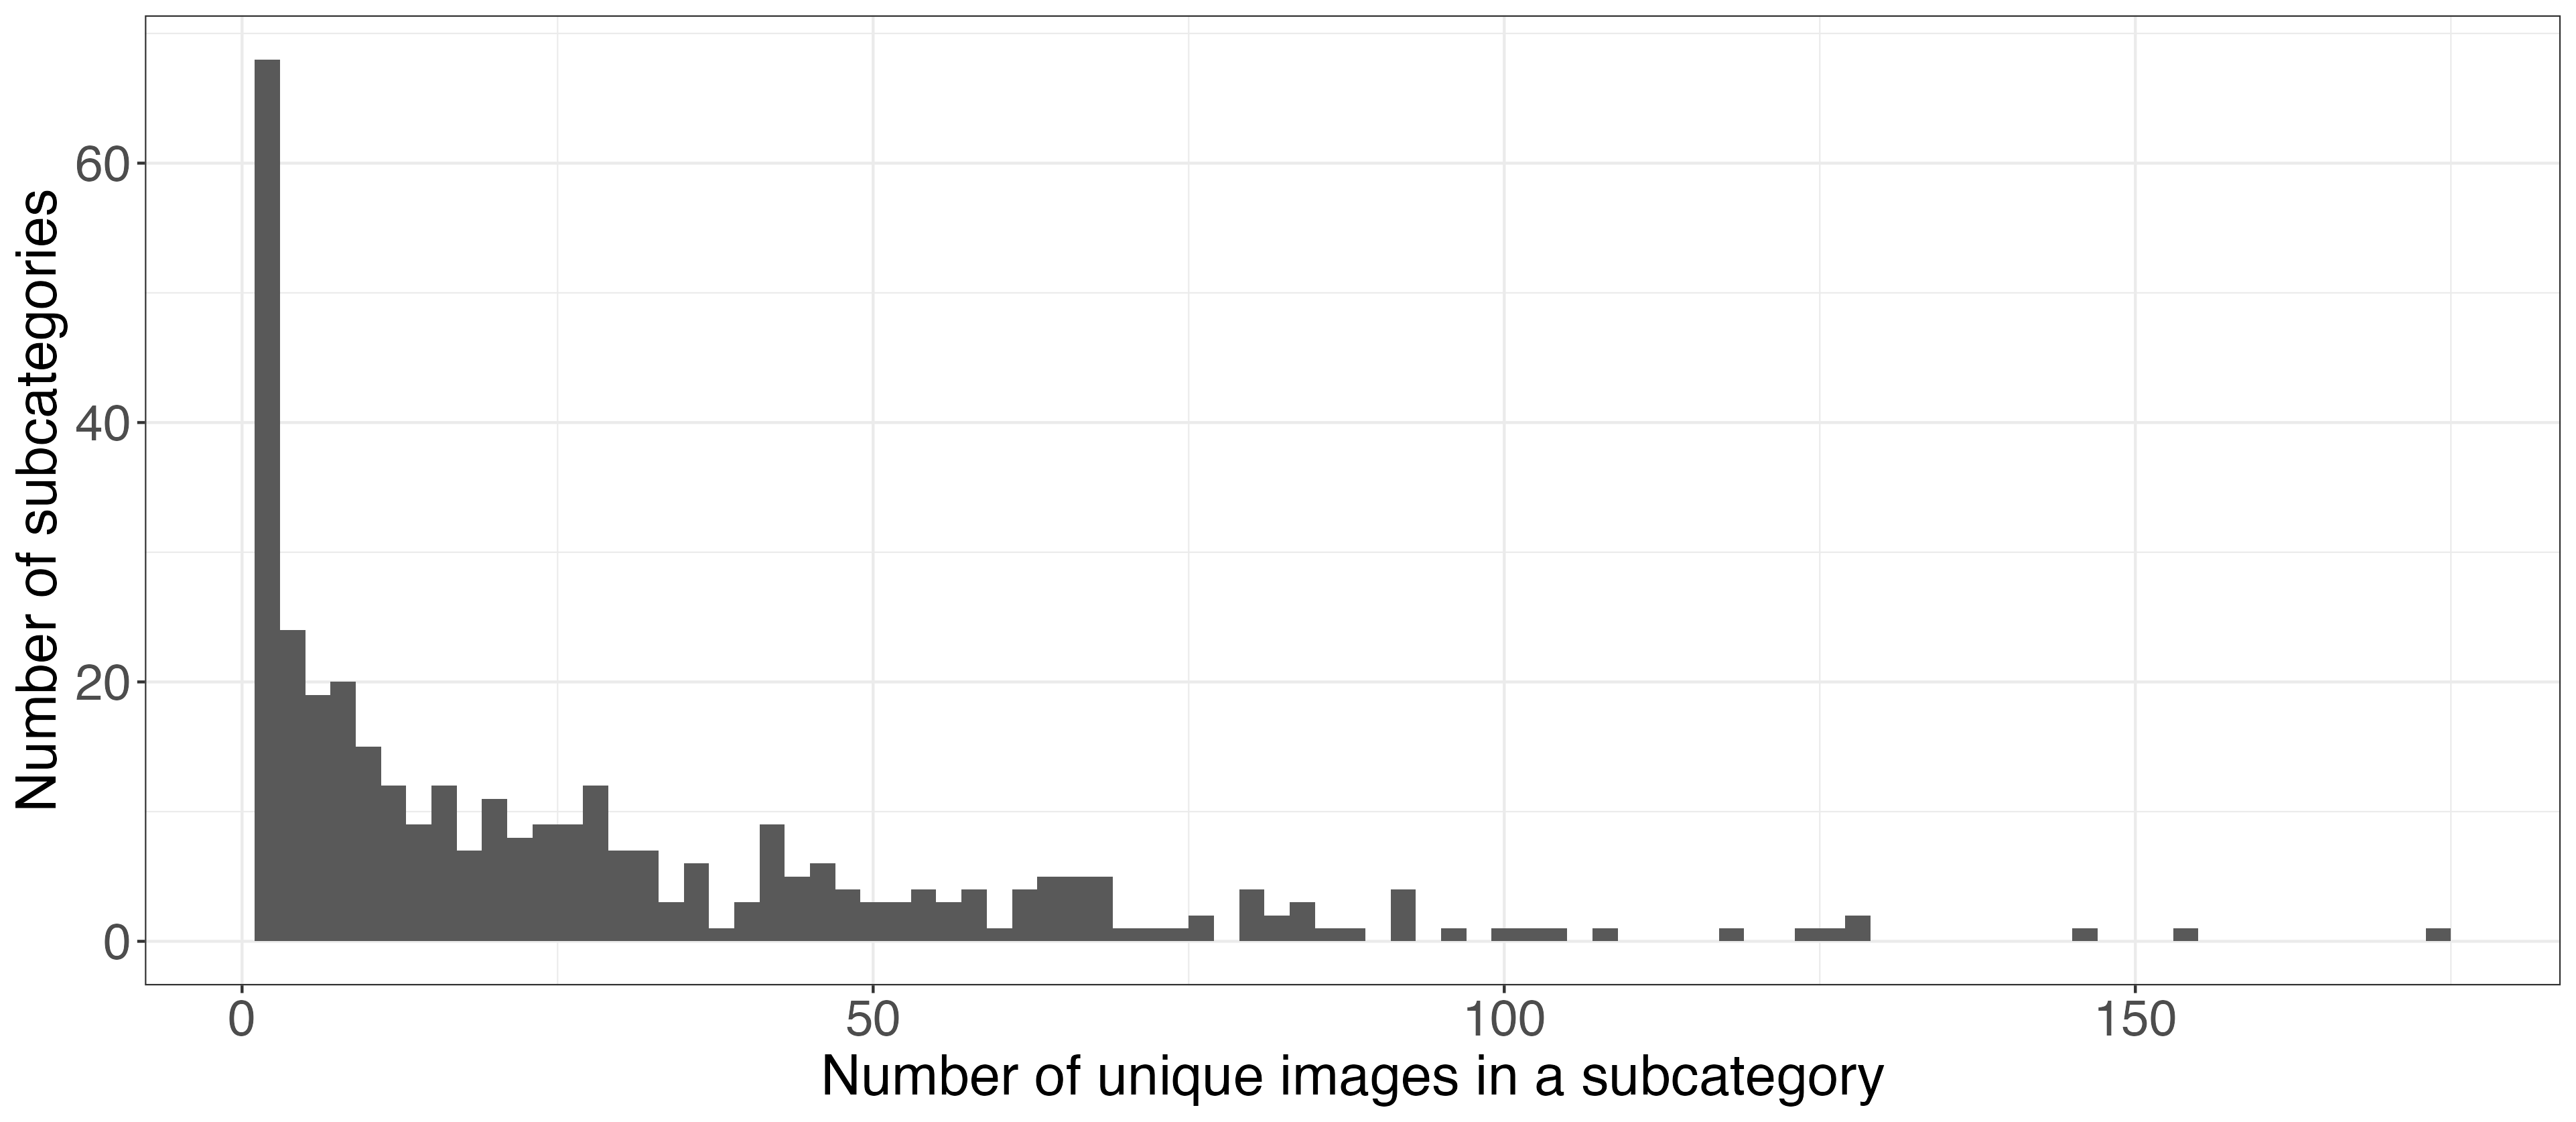
\includegraphics[width = \textwidth]{../figs/Subcategory_Distinct_Image_Dist.png}
    \caption{Distribution of the number of distinct images per subcategory. One
    can see that the distribution is right-skewed and that a lot of
    subcategories consist of only a few distinct images.}
    \label{fig:subcategory_distinct_image_dist}
\end{figure}

\subsection{Modelling Labelling Uncertainty}
We can express the MLE of the confusion matrix $\Theta$ from equation
\ref{eq:theta_mle} using matrix notation. We define the matrix $\bY$ as the $n
\times K$ matrix with the vote distributions $\bY^{(i)}$ as rows. We define the
matrix $\bZ$ as the $K \times n$ matrix with the $\bZ^{(i)}$ as columns.
Furthermore, we define the vector $\bJ$ as the $n \times 1$ vector with the
$J^{(i)}, i = 1,\dots, n$ as entries. We can then write the MLE of the confusion
matrix $\Theta$ as
\begin{equation}
    \hTheta = \bZ \bY \cdot \text{diag}(\bZ \bJ)^{-1}
    \label{eq:theta_mle_matrix}
\end{equation}

\subsection{Sources of Uncertainty}
\begin{figure}[H]
    \centering
    \includegraphics[width = \textwidth]{../figs/confusion_matrices_comparison_subcategories_entropy.png}
    \caption{Sources of uncertainty in the labelling process.}
    \label{fig:confusion_matrices_comparison_subcategories_entropy}
\end{figure}